\section{Theory}
	A lock-in amplifier, as its name suggests, is used for phase-sensitive detection and amplification of small AC voltages. Its maximum DC output is achieved when the signal being measured is in phase with a reference signal. As a result, the output signal's bandwidth is fixed in a specific phase (small range) that coincides with the input signal's phase. The frequency range in which this lock-in amplifier can operate is $100 Hz$ to $5 kHz$. A DC output of about $1V$ is produced by an AC signal with an amplitude of $200 rms$.

	\subsection{Components of Lock-In Amplifer and its working}
		The front panel of the Lock-in Amplifier is divided into two pieces. The main switch is located in the top left corner of the front panel and is indicated by an indicator light when depressed. Three banana temrinals are also located on the left side. Two toggle switches are present. One can internally calibrate the lock-in when both are set to the CAL mode. The toggle switches are set to EXT when measuring an external signal. The two Banana terminals (Red and Black) at the front panel's bottom should be connected to the external AC signal in this mode. The RCA socket labelled EXT REF should receive the external reference signal.

		There are several RCA sockets on the front panel's right side. A signal generator is connected to the SIG GEN socket at the bottom to calibrate the lock-in amplifier internally. We have two additional sockets with the labels REF and REF' above the sig gen RCA socket. These are sockets that can be used to display the reference signal and the phase-shifted reference signal on a two-channel oscilloscope, respectively. The PHASE SHIFT ADJUST pot's knob is used to adjust the phase shift between the reference and input signals. To display the amplified small AC signal with noise, connect an oscilloscope to the RCA socket labelled SIGNAL. The RCA socket marked PIN 13 shows the output at pin 13 of the chip AD 630. On an oscilloscope, the pattern of the output at pin 13 changes as the phase shift adjust knob is turned. The output at Pin 13 resembles a full wave rectifier's output when the phase-shifted reference and the signal are in phase. A DMM in the proper DC range is attached to the RCA pin with the label "OUTPUT." This instrument measures the Lock-in chip's pin 13's amplified DC output. The block diagram of the LIA is given below:

	
		\begin{figure}[H]
			\centering
			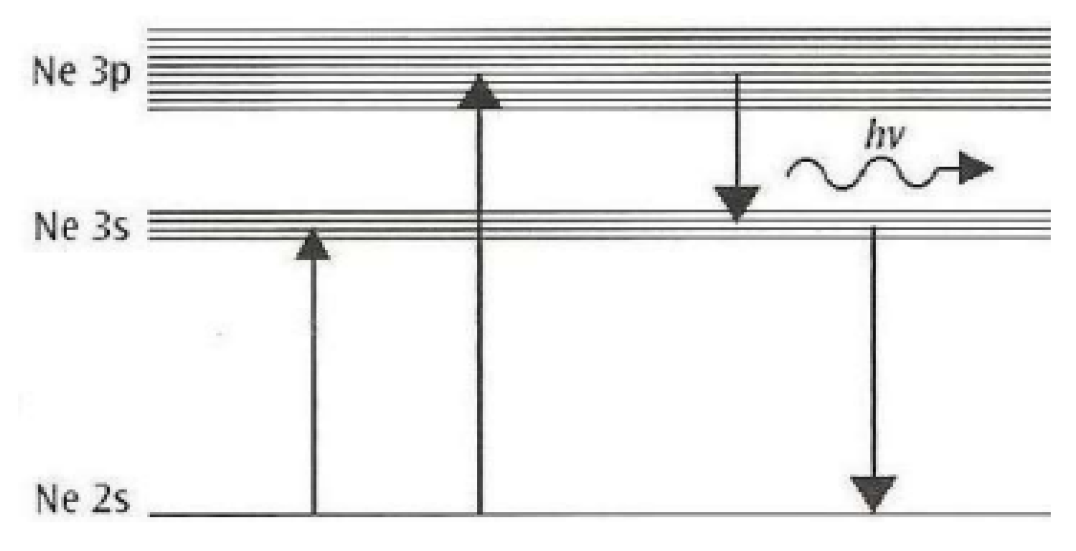
\includegraphics[width=0.45\textwidth]{1.png}
			\caption{Schematic Diagram of Lock In Amplifier Circuit}
			\label{fig:1}
		\end{figure}
	
	\subsection{Principle of Phase sensitive Detection}

		Amplifiers are used to amplify a weak AC signal while limiting the amount of noise amplification. Amplification by itself won't help us distinguish the signal from noise if the signal is very weak. Flicker noise is one of the many types of noise, and its power spectrum is inversely proportional to the frequency of the signal. Only when one works at extremely low frequencies does this noise become an issue. The noise caused by electromagnetic pick up from operating motors and tube lights is another problem, but it can be reduced by using electromagnetic shielding. Then there is thermal noise, which has electromagnetic origins and is influenced by the circuit's current and resistance. Lower currents significantly reduce the amount of thermal noise. The range of its power encompasses all frequencies. So it is called white noise. To reduce this noise we either reduce the temperature T or reduce the bandwidth W of the amplifier. For detecting very weak signals at room temperature we have to effectively reduce the bandwidth to a few Hertz though the amplifier has a large bandwidth in kilohertz range. Phase sensitive detection is used for locking in the phase of the output signal to a narrow bandwidth with respect to the reference signal.

		The LIA receives an AC sinusoidal input voltage for phase-sensitive detection. The source could come from a signal generator, a mutual inductance's primary coil current, etc. It might be a periodic intensity-modulated light signal. This cause will result in an effect that may differ in phase from the cause but will have the same frequency as the cause. The induced emf in the secondary coil is the result of mutual inductance. The effect will only be a few microvolts or nanovolts, but when amplified, it will result in significant noise. To get around this, we must take a reference signal and reduce the bandwidth. We use a reference signal that is derived from the cause signal and is in phase with it to cancel out the noise in relation to the weak effect signal. For instance, in an inductance, the primary coil and a resistance are connected in series so that any current flowing through the primary also flows through the resistance R. The reference signal will be the voltage applied across the resistance. One can produce a reference signal of a few tens of millivolts or more by selecting R properly.

		Let the phase difference between the reference signal and input signal be $\phi$. We have:


		$$V_{signal} = V\sin\omega t + \phi$$
		$$V_{ref} = V\sin\omega t$$
		
		These signals are then fed to the phase-sensitive detector chip AD630. A direct amplifier and an inverse amplifier, both of which are identical, are present in this chip. This indicates that the output and input are in phase. The output of the other amplifier, which is an inverse amplifier, is $180^\circ$ out of phase with the input. There is a switch that a comparator controls. the reference signal is picked up by the comparator. Due to the amplification:
		
		$$V_{out} = \mu V_{signal} \;\;\;\;\;\; [0<t<\sfrac{T}{2}]$$
		$$V_{out} = \mu V_{signal} \;\;\;\;\;\; [\sfrac{T}{2}<t<T]$$

		where $\mu$ is the amplification factor. The DC voltage can be calculated by integrating for a time period to give:

		$$V_{DC} = \frac{4\mu v_0 \cos\phi}{2\pi}$$

		This demonstrates that the output power will be at its highest when the signal voltage is in phase with the reference signal, meaning that only a small bandwidth locked in this phase will produce a significant output. Because we make the weak signal lock in phase with the phase-shifted reference to provide the highest possible DC output voltage, we refer to this phase sensitive detection and the amplifier as a lock-in amplifier.
	
	\subsection{Mutual Inductance with Lock-In Amplifier}
		When two coils are placed side by side and an AC current is run through the primary (also known as the first coil), the second coil induces an AC voltage at the same frequency. When the primary current changes as follows:

		$$I = I_0 \sin\omega t$$

		The voltage in the secondary coil is given by:

		$$V = -MI_0\sin\omega t + \sfrac{\pi}{2}$$

		The amplification is greatest when the signals inside the LIA are at a $90^\circ$ phase difference because the phase difference between the primary current and the induced emf is $\frac{pi}{2}$ and the primary voltage serves as the reference signal for the secondary signal. The induced is proportional to both the frequency $f$ and the current amplitude $I_0$.

		The mutual inductance $M$ is given by:

		\begin{equation}
			M = \frac{R\beta}{2\pi}
			\label{eq:1}
		\end{equation}

		R is the resistance in the primary circuit $4.8 k\ohm$.
	
	\subsection{Measurement of Low Resistance}
		Measurement of low resistance (resistance less than an Ohm) with the DC technique would require a high current. Also since the voltage developed across the resistance will be small, it will be affected by noise when it is amplified. In this box a resistance of $4.7 k (1/4 W)$ is connected with the low resistance and a 100-Ohm $(1/4 W)$ resistor. The free end of the $4.7k$ resistor is connected to the red banana terminal, the free end of the low resistance to the middle terminal (Green). A $100ohm$ resistor is connected to the middle terminal (Green) and the end terminal (in the above box this terminal is yellow). Potential leads across the low resistance come to the RCA socket marked signal on the left top of the box. The voltage across the $100ohm$ resistor serves as the reference signal. This reference signal can be taken between the middle and end banana terminals on the box or from the RCA socket marked reference at the right top of the box.
	
		\begin{figure}[H]
			\centering
			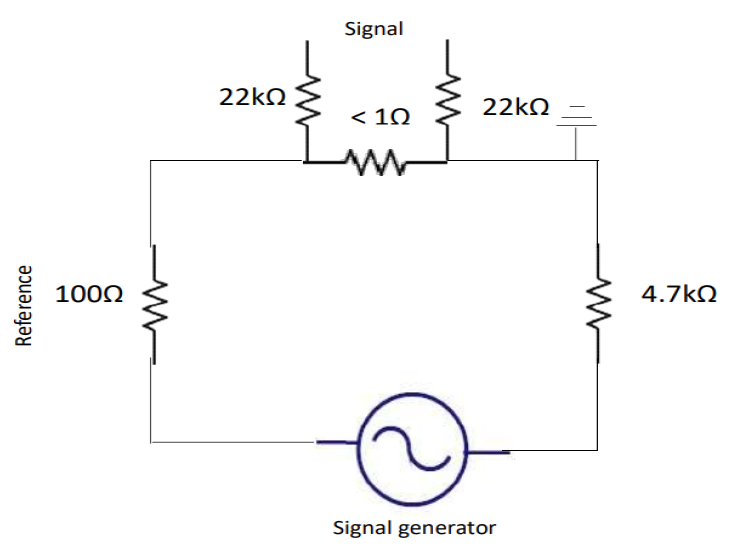
\includegraphics[width=0.45\textwidth]{2.png}
			\caption{The Resistance Circuit}
			\label{fig:2}
		\end{figure}

		The output DC voltage and input AC voltages are tabulated and the slope is found. On solving we get the following relation between the slope $\alpha$ and resistance r:

		\begin{equation}
			\alpha = \frac{\mu r}{R}
			\label{eq:2}
		\end{equation}
